
% This is the main file to setup the document.
% Document organization and appearance settings are all done here
% Each chapter is a separate tex file, all linked together here


% Preamble (document settings) -----------------------------------------------------------
% Document type and font --
\documentclass[10pt]{report}
\usepackage[utf8]{inputenc} %utf-8 encoding for ASCII symbols

% insert packages here --
\usepackage{graphicx}       %for handling images

\usepackage{amsmath}        %for math symbols

\usepackage{breakcites}     %to avoid citations extending into the margin

\usepackage[margin=1in]{geometry}   %to reduce margins to 1 inch, default margins wasted a lot of space

\usepackage{sidecap}        %to enable side captions on figures

\usepackage{setspace}       %to enable doublespacing   

\usepackage[
backend=biber,
style=apa,
citestyle=apa
]{biblatex}       %use the biblatex package

\addbibresource{mybibfile1.bib}   %path to the bib file


\usepackage{hyperref}       % to create a linked table of contents
\hypersetup{
    colorlinks,
    citecolor=black,
    filecolor=black,
    linkcolor=black,
    urlcolor=black
}

% Set path to images
\graphicspath{ {images/} }  % Direct to the main image folder, always good to create sub-folders to organize images for individual chapters

\singlespacing  %making text double spaces

% End of preamble
%-------------------------------------------------------------------------------------------
\begin{document}

% Making title page


\begin{titlepage}
   \begin{center}
   \begin{doublespacing}

       \begin{figure}
       \centering
       
\includegraphics[width=0.7\textwidth]{images/MUN_Logo_RGB.png}
       \end{figure}
       
       
       \vspace*{5mm}
       {\large\textbf{CMSC6950 COURSE PROJECT}}

       %\textbf{DOCTOR OF PHILOSOPHY}
       \vspace{30mm}
       
       {\Large\textbf{WINDROSE APPLICATION}}

    
            
       \vspace{30mm}

       {\Large\textbf{SHUO WANG}\\
       %\textbf{}
       }

       \vfill
       {\large \textbf{Department of Computer Science}\\
       \textbf{August, 2020}}
       
    \end{doublespacing}

   \end{center}
\end{titlepage}


% Starting frontmatter:
% Abstract goes here
\doublespacing
 \thispagestyle{plain}
\begin{center}
    \Large
    \textbf{Windrose Application}
        
    \vspace{0.4cm}
    \textbf{Shuo Wang}
    
    \vspace{0.4cm}
    \large{Supervisor: Prof James Munroe}
       
    \vspace{0.9cm}
    \textbf{Abstract}
\end{center}

Abstract text goes here.. 

\pagenumbering{roman}   % Roman page numbering to start from abstract onwards

\singlespacing          % keep pre-content single spaced
\listoffigures          % generate list of figures
% \listoftables           % generate list of tables

% End of frontmatter

% Insert table of contents
 \tableofcontents

% Main matter starts here --
% Inserting individual chapters. Mention chapter titles here and simple link the chapter's tex file

 \chapter{Introduction}     % Mention chapter title here
  \pagenumbering{arabic}    % We want Arabic numerals for main matter page numbering
 
\section{Wind rose}

A wind rose is a graphic tool used by meteorologists to give a succinct view of how wind speed and direction are typically distributed at a particular location. Historically, wind roses were predecessors of the compass rose, as there was no differentiation between a cardinal direction and the wind which blew from such a direction. Using a polar coordinate system of gridding, the frequency of winds over a time period is plotted by wind direction, with color bands showing wind speed ranges. The direction of the longest spoke shows the wind direction with the greatest frequency(\cite{wikipedia}). \par

% \textcite{parish2009propagation}

\section{Data source}
The wind data is obtained directly from the SmartAtlantic Alliance which is an initiative of the Fisheries and Marine Institute of Memorial University of Newfoundland's Centre for Applied Ocean Technology (CTec) and the Centre for Ocean Ventures and Entrepreneurship (COVE) of Halifax.\par
The URL of CSV data file can be generated from their website as the figure shown below.\par

\begin{figure}[h!]
    \centering
    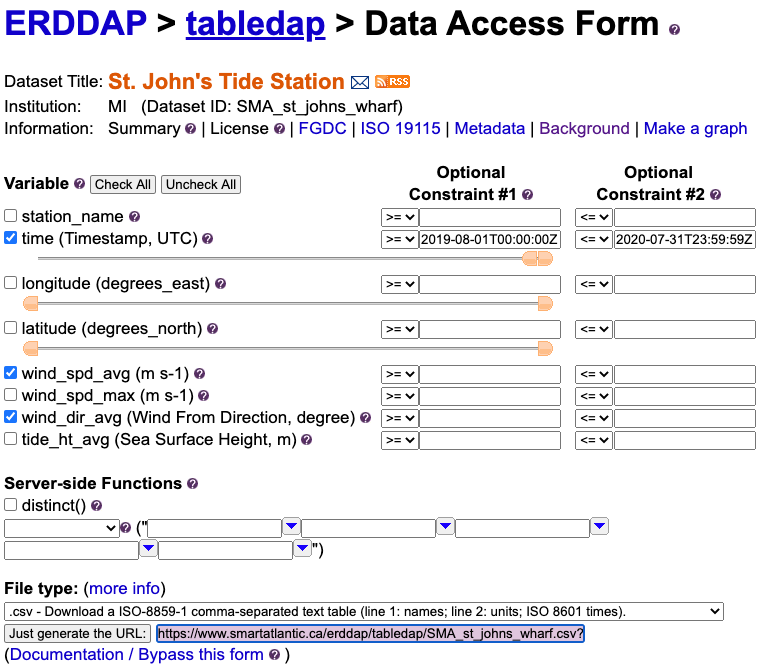
\includegraphics[width=0.50\textwidth]{images/data_source.png}
    \caption{URL generation of CSV data file}
    \label{fig: PaleBlueDot}    
\end{figure}

In this project, the information of timestamp, wind speed and wind direction in the last 365 days (from 1 August 2019 to 31 July 2020) was collected and used to plot wind rose.\par

\section{Analysis workflow}
 % Link to the chapter tex file


\chapter{Data management and analysis}


In this chapter we will look at..

\section{Some section}

\subsection{Subsection}
Backup your bullshit (and data)..

 \chapter{Data Visualization}
 In this chapter we will look at..

\section{Some section}

\subsection{A basic scatter plot with transparency}

% Insert images like this:
\begin{figure}[h!]
    \centering
    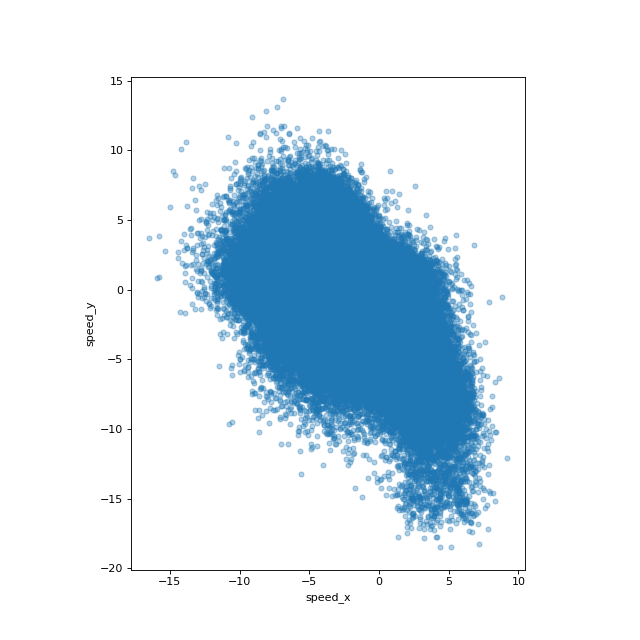
\includegraphics[width=0.50\textwidth]{images/figure1.png}
    \caption{some description about the figure1}
    \label{fig: PaleBlueDot}    
\end{figure}

  \chapter{Some chapter}
 This is yet another chapter.

\section{Some section}

\subsection{Subsection}
Always use vectorized graphics. Black and white plots with different markerstyles \textgreater multicolor plots 
 
 \chapter{Planning and Conclusion}
 This seems to be the last chapter in this report..

\section{Some section}

\subsection{Subsection}
Nobody will read your QE report.

    
% Include appendix      % Set this up if needed
%\appendix

% Insert bibliography here
\printbibliography

\end{document}

% End of document
%-----------------------------------------------------------------------------------------------------